\documentclass[titlepage]{article}
\usepackage[upright]{fourier}
\usepackage[utf8]{inputenc}
\usepackage[english]{babel}
\usepackage[margin=1in]{geometry}
\usepackage[T1]{fontenc}

\usepackage[colorlinks=true,linkcolor=teal]{hyperref}
\usepackage{amssymb,amsmath,minted,float,graphicx,textcomp,systeme,listings,physics,mathtools,ifthen,esvect,hyperref,fancyhdr,lastpage,marginnote,chngcntr,fancyvrb,subcaption,svg}

\usepackage[backend=biber,style=numeric]{biblatex}
\addbibresource{article.bib}

\DeclareMathOperator{\e}{e}
\def\mathbi#1{\textbf{\em #1}}

\setlength\parindent{0pt}

%%%%%%%%%%%% PARAMETRES
\newcommand{\UE}{4XX}
\newcommand{\type}{}%TD-TP-COURS
\newcommand{\nb}{0}%nb 
\newcommand{\sbt}{}%soustitre
\author{Gabriel ROBERT-DAUTUN}
\date{Mars 2022}

% mise en page (header, compteur, fancy)
\pagestyle{fancy}
\lhead{Dynamic image reconstruction}
\rfoot{\thepage /\pageref{LastPage}}
\lfoot{}
\cfoot{}
\renewcommand{\footrulewidth}{0.4pt}

%reset compteur section par partie
\counterwithin*{section}{part}

% permet notes + simples en marge à gauche (eg compteur de question)
\reversemarginpar
\newcommand{\mgn}[1]{\marginnote{#1}}

%sinon warning mdr
\setlength{\headheight}{13.07225pt}

\newcommand{\hinv}[1]{#1^{\circ-1}} % inverse de hadamard
\newcommand{\fnorm}[1]{|\vert#1|\vert_{F}} % norme de Frobenius
\newcommand{\moy}[1]{\boldsymbol{\mathsf{m}}_{#1}}
\newcommand{\autocorr}[1]{\expval{(#1)(#1)^H}}
\newcommand{\ccorr}[2]{\expval{(#1)(#2)^H}}

\renewcommand{\expval}[1]{\text{E}\left[#1\right]}
\newcommand{\w}{\boldsymbol{w}}
\renewcommand{\v}{\boldsymbol{v}}
\newcommand{\Q}{\boldsymbol{\mathsf{Q}}}
\newcommand{\R}{\boldsymbol{\mathsf{R}}}
\renewcommand{\H}{\boldsymbol{\mathsf{H}}}
\newcommand{\A}{\boldsymbol{\mathsf{A}}}
\newcommand{\I}{\boldsymbol{\mathsf{I}}}
\newcommand{\K}{\boldsymbol{\mathsf{K}}}

\newcommand{\x}{\boldsymbol{x}}
\newcommand{\y}{\boldsymbol{y}}
\newcommand{\z}{\boldsymbol{z}}

\newcommand{\dz}{\Delta\boldsymbol{z}}

\newcommand{\xp}{\widehat{\x}_{k|k-1}}
\newcommand{\xa}{\widehat{\x}_{k-1|k-1}}
\newcommand{\xe}{\widehat{\x}_{k|k}}
\newcommand{\yp}{\widehat{\y}_{k|k-1}}

\newcommand{\Pp}{\boldsymbol{\mathsf{P}}_{k|k-1}}
\newcommand{\Pa}{\boldsymbol{\mathsf{P}}_{k-1|k-1}}
\newcommand{\Pe}{\boldsymbol{\mathsf{P}}_{k|k}}
\renewcommand{\P}{\boldsymbol{\mathsf{P}}}

\newcommand{\vbeps}{\boldsymbol{\varepsilon}}
\newcommand{\C}{\mathcal{C}}
\newcommand{\D}{\mathcal{D}}

\title{%
	Radioastronomical image reconstruction using Kalman filter under ionospheric perturbations}

\begin{document}
	
	\begin{titlepage}
	
	\vspace*{.3\textheight}
	\huge
	\centering
	\textbf{Dynamic radioastronomic image reconstruction using Kalman filter under ionospheric perturbations}
	
	\vspace{1cm}
	\LARGE
	G. Robert-Dautun
	
	\vfill
	\large
	Supervised by I. Vin
	
	\vspace{0.8cm}
	
	\Large
	Satie\\
	France\\
	July 2022
	
	\end{titlepage}
	
	\newpage
	\tableofcontents
	
		\newpage
	\part{SATIE}
	
	SATIE stands for \emph{laboratoire des Systèmes et Applications des Technologies de l'Information et de l'Energie} (Information and Energy Technology Systems and Applications Laboratory).\\
	Created in 1975 under the name \emph{Laboratoire d'Electricité de l'ENSET}, then renamed \emph{LESiR} in 1984 at the time of its association with CNRS, then finally SATIE in 2002, the laboratory covers a large field of study including signal processing, electronics, and energy conversion.\\
	
	The SATIE is linked to the following academic structures : ENS Paris-Saclay, ENS Rennes, Université Paris-Saclay, Cergy Paris Université, Université Gustave Eiffel, CNAM Paris and CNRS. It counts five geographical sites near the aforementioned structures. 
	
	\begin{figure}[H]
		\centering
		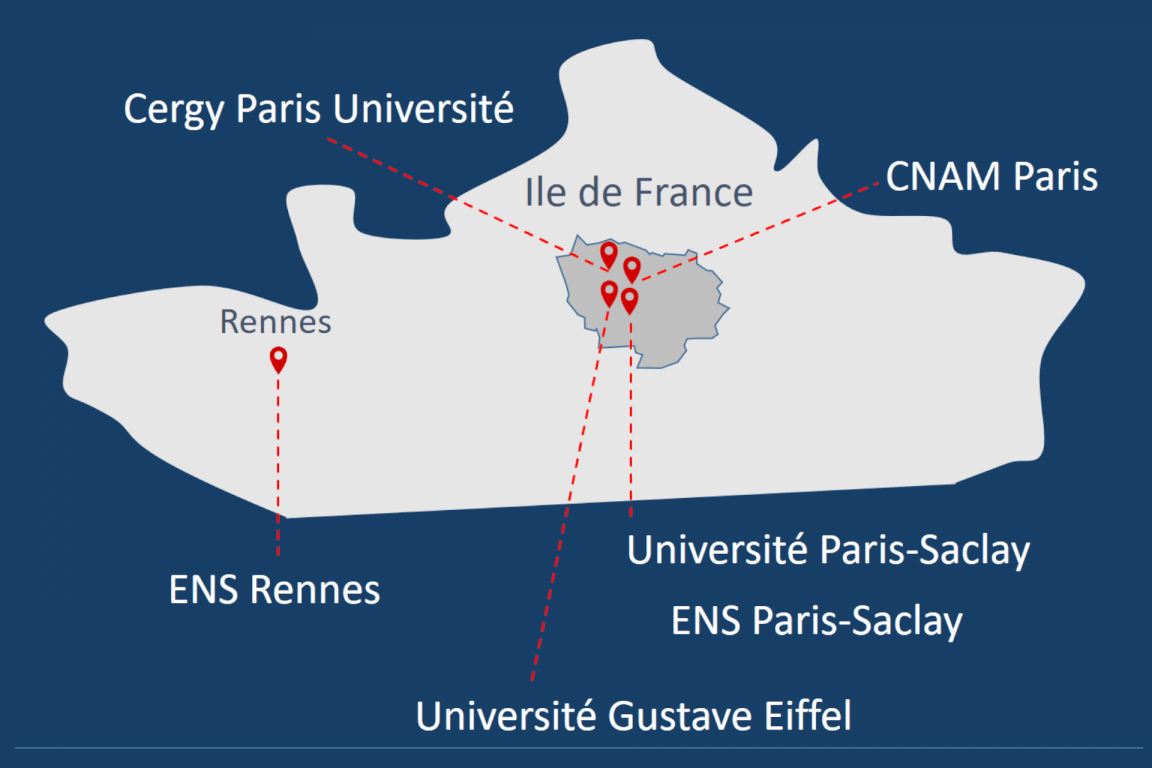
\includegraphics[width=0.7\linewidth]{src/sites_geoo_satie}
		\caption{Geographic sites of SATIE (copyright E. Vourc'h)}
		\label{fig:sitesgeoosatie}
	\end{figure}
	
	Research in SATIE is dispatched around two main divisions :
	
	\begin{tabular}{|c||c|c|} % a traduire ffs
		\hline
		Divisions & Components and Systems for electrical energy & Multi-scale information and analysis systems \\ & (CSEE) & (SIAME) \\\hline
		Research fields & \begin{tabular}{@{}c@{}}
			Materials: from synthesis to application\vspace{8px} \\ Power electronics: integration, \\ usage constraints, interfaces\vspace{8px} \\ Transducers and energy systems: \\ methodologies, design and control
		\end{tabular} & \begin{tabular}{@{}c@{}}
			Instrumentation and imagery\vspace{5px} \\ Methods and tools for signals and systems\\ (MOSS)
		\end{tabular}
		\\\hline
	\end{tabular}
	\vspace{7px}\\
	I did my internship in the SIAME/MOSS division. \\
	The SIAME/MOSS division is focused on getting a better understanding and mastering complex systems. The three main topics of the division are :
	\paragraph{Data and image analysis:} this topic's main goal is to estimate physical or semantic quantities from observations data. This data is incomplete, inaccurate, and not absolutely reliable. When data is generated using multi-sensor systems, it presents similarities and complementarities that can be used to get better estimations.
	
	\newpage
	\part{Introduction}
	
	When observing distant objects, instruments resolution matters the most. When using optical telescopes, the determining factor for resolution is the size of the primary mirror. When observing really distant objects, the required size to have a decent resolution becomes unrealistically big. To address this problem, radio interferometry replaces a single optical instrument with multiple antennas collecting electromagnetic waves. When gathering these measures together, we can obtain a better angular resolution than any real single optical instrument could get. \\
	
	Those distant objects are not fixed in time and a lot of calculations have been done to create evolution models for them. The goal here is not to use observations to confirm models, but to assume a model is known and get better results considering the knowledge of both observations and model. \\ 
	
	A (non extended) Kalman filter is a linear quadratic estimator, using observations, state-transition model and knowledge about noise and errors to compute a more accurate result than observations alone. Radio astronomical measures being prone to noise and errors, usage of this filtering method seems \emph{a priori} a good way to improve accuracy of reconstruction. \\
		
	A sensitive part of the filter is the observations model, needing precise knowledge of antennas positions and directions. A of this goal work is to determine how inaccuracies in these measurements affect image reconstruction, and if it is realistically usable in radio astronomical imagery. \\
	
	\newpage
	\part{Notations and problem}
	\section{Notations}
	
	\subsection{General notations}
	
	$\expval{\bullet}$ denotes the expected value of a random variable/vector/matrix.\\
	
	Bold symbols represent vectors, normal ones represent scalars except when stated otherwise.\\
	
	Operator $\moy{\bullet}$ represents the mean value/vector/matrix of the given $\bullet$ set.\\
	
	When a 2-D matrix element is indexed with a single coordinate, it designates the reshaped matrix in a 1-D vector.\\
	
	$\mathbb{I}$ is the identity matrix.
	
	
		\subsection{Hadamard product}
	
	%On introduit la notation $\odot$ associée au produit de Hadamard, qui effectue la multiplication élément à élément de deux matrices de même taille :
	Hadamard product, denoted $\odot$, is the element-wise product of same sized matrices :
	
	$$
	\forall (A,B)\in\left(\mathbb{C}^{m\times n}\right)^2, \quad A\odot B\in\mathbb{C}^{m\times n} \quad\text{and}\quad \forall (i,j)\in\llbracket1;m\rrbracket\times\llbracket1;n\rrbracket,\, (A\odot B)_{i,j} = A_{i,j}\times B_{i,j}
	$$
	
	%On introduit également l'inverse de Hadamard, qui inverse élément par élément une matrice
	We can further introduce Hadamard inversion :
	$$
	\forall A \in \left(\mathbb{C}\backslash\{0\}\right)^{m\times n},\quad \hinv{A}\in\left(\mathbb{C}\backslash\{0\}\right)^{m\times n} \quad\text{and}\quad \forall (i,j)\in\llbracket1;m\rrbracket\times\llbracket1;n\rrbracket,\, \left(\hinv{A}\right)_{i,j} = \left(A_{i,j}\right)^{-1}
	$$ 
	
%	Ainsi que la notation $\oslash$ désignant la division de Hadamard :
	And notation $\oslash$ being Hadamard division :
	$$
	\forall (A,B)\in\mathbb{C}^{m\times n}\times\left(\mathbb{C}\backslash0\right)^{m\times n}, \quad A\oslash B\in\mathbb{C}^{m\times n} \quad\text{and}\quad \forall (i,j)\in\llbracket1;m\rrbracket\times\llbracket1;n\rrbracket,\, (A\oslash B)_{i,j} = \frac{A_{i,j}}{B_{i,j}}
	$$
	
	\subsection{Norms and distances}
	
	%On dénote $\fnorm{\bullet}$ la norme de Frobenius :
	In order to compute distances between matrices, we note $\fnorm{\bullet}$ Frobenius norm :
	$$
	A\in\mathcal{M}_{m,n}(\mathbb{K}) \quad \fnorm{A} := \sqrt{\tr{AA^H}} = \sqrt{
		\;\;\;\sum_{
			\mathclap{
				\substack{
					1\le i\le m \\1\le j\le n
				}
			}
		}\abs{A_{ij}}^2}
	$$
	
	%Qui induit sur $\mathcal{M}_{m,n}(\mathbb{D})$ la distance normalisée $d_1$ :
	Inducing the distance $d_1$ :
	$$
	\forall(A,B)\in\left(\mathcal{M}_{m,n}(\mathbb{K})\right)^2\quad d_1(A,B) = \frac{\fnorm{A-B}}{mn}
	$$
	
	%Ainsi que la distance $d_2$ :
	In order to measure influence of a specific element, the additive distance $d_2$ is the following :
	$$
	\forall(A,B)\in\left(\mathcal{M}_{m,n}(\mathbb{K})\right)^2\quad d_2(A,B) = \sum_{
		\mathclap{
			\substack{
				1\le i\le m \\1\le j\le n
			}
		}
	}\abs{A_{ij} - B_{i,j}}
	$$
	
	\section{Measure and parameters}
	
	In order to measure precisely the effects, the following parameters will be used :
	\begin{itemize}
		\item The antennas distribution is a 8.57m square 6$\times$6 grid. The number of antennas is thus $J = 36$
		\item The observed directions grid is a 10$\times$10 square. The number of directions is thus $D=100$
		\item A normally distributed observation noise will be introduced with Signal to Noise Ratio (SNR) of 10. 
		\item The first image used for Kalman will be computed using Minimum Variance Distortionless Response (MVDR) method \cite{bible}, deconvoluted with Maximum Entropy Method (MEM) \cite{MEM}
		\item Measured wavelength is $\lambda =0.3$m
	\end{itemize}

	The following matrices and sets will be used to describe this setup :
	\begin{itemize}
		\item $\z$ represents the positions of each antenna in the 2-D grid
		\item $\dz_{ij}$ is the baseline : $\dz_{ij} = \z_i - \z_j$. 
		\item $\I$ is the directions matrix, represented as normalised direction cosines.
	\end{itemize}
		
	\section{Evolution model and Kalman filtering}
	
	We consider a set $\{\x_k\}$ of $n$ vector as theoretical images taken at a regular time interval. Those images are measured by an antenna mesh $\{\z_k\}$ which UV plane will be written $H$, more generally written as observation model. Measurements vectors will be designated by $n$ measures $\{\y_k\}$.\\
	$\H$ can be computed by the following :
	\begin{equation}
		\H_{j,q} = \exp(-i\frac{2\pi}{\lambda}\dz_{j}\dotproduct\I_q)
	\end{equation}
	We will consider the following model to describe time evolution and observation equation :
	$$
		\begin{cases}
			\x_k = \A\x_{k-1} + \w_{k-1}\\
			\y_k = \H\x_k + \v_k
		\end{cases}
	$$
	
	Where :
	\begin{itemize}
		\item $A$ is the linear state-transition model between time $k-1$ and $k$, assuming evolution is time invariant
		\item $\{\w_k\}$ is the state noise sequence
		\item $\{\v_k\}$ is the measurements noise sequence
	\end{itemize}
	
		
	In order to build images dynamically with better precision, a Kalman filter has been implemented.\\
	
	This filter requires more inputs to estimate the state of the system :
	\begin{itemize}
		\item $\{\Q_k\}$, the covariance of the process noise sequence
		\item $\{\R_k\}$, the covariance of the observation noise sequence
	\end{itemize}

	Which can be rewritten as
	$$
		\begin{cases}
			\Q_k = \expval{\w_{k-1}\w_{k-1}^H} - \expval{\w_{k-1}}\expval{\w_{k-1}}^H \\
			\R_k = \expval{\v_{k}\v_{k}^H} - \expval{\v_k}\expval{\v_k}^H 
		\end{cases}
	$$
	
	Those inputs are not \emph{a priori} known, but it has been shown that using the \emph{autocovariance least-squares} (ALS) method provides a good estimate of those matrices. [CITATION NEEDED] \\
	We will assume that these inputs are known perfectly except when specified otherwise.\\
	
	Kalman filtering works in 2 steps :
	\paragraph{Prediction} : This step predicts the state of the system at next time-step through de transition-state model, and the predicted measurement :
	$$
	\begin{cases}
		\xp = A\xa + \moy{\w_k}\\
		\yp = H\xp + \moy{\v_k}
	\end{cases}
	$$
	And the covariance matrix :
	$$
		\Pp = \autocorr{\xp - \x_k} = \A\Pa \A^H + \Q_k
	$$
	This result can be computed using least-square estimation of the prediction error covariance\cite{intro_KF}
	
	\paragraph{Update} : Using prior knowledge about noise and observation model, the main goal is to build an image from both prediction and measurement using maximum likelihood estimation in order to enhance the resulting image. This can be written as looking for $K_k$, known as \emph{Kalman gain}, such as :
	\begin{equation}
		\xe = \xp + K_k\left(\y_k - \yp\right)
	\end{equation}
	
	minimises the quadratic error :
	\begin{equation}
		K_k = \arg\min_K \Pe = \arg\min_K \autocorr{\xe - \x_k}
	\end{equation}
	
	The resulting expression for $K_k$ is \cite{intro_KF} :
	\begin{equation}
		K_k = \Pp H^H\left(H\Pp H^H + \R_k\right)^{-1}
	\end{equation}

	Thus the update phase can be written :
	\begin{equation}
		\begin{cases}
			\xe = \xp + K_k\left(\y_k - \yp\right) \\
			\Pe = \left(\mathbb{I} - K_kH\right)\Pp
		\end{cases}
	\end{equation}
	
		\section{Data simulation and Image reconstruction}
	\subsection{Simulation}
	
	In order to simulate data, an image is introduced as the "reference image", this image will only be used in order to compute simulated observations. The selected picture must respect the following conditions :
	\begin{itemize}
		\item mostly black background, to give realistic results for space imagery
		\item no convolution effect, as all directions are considered sources of different intensities, only real sources must appear
	\end{itemize}
	The following picture is the one used :
	
	\begin{figure}[H]
		\centering
		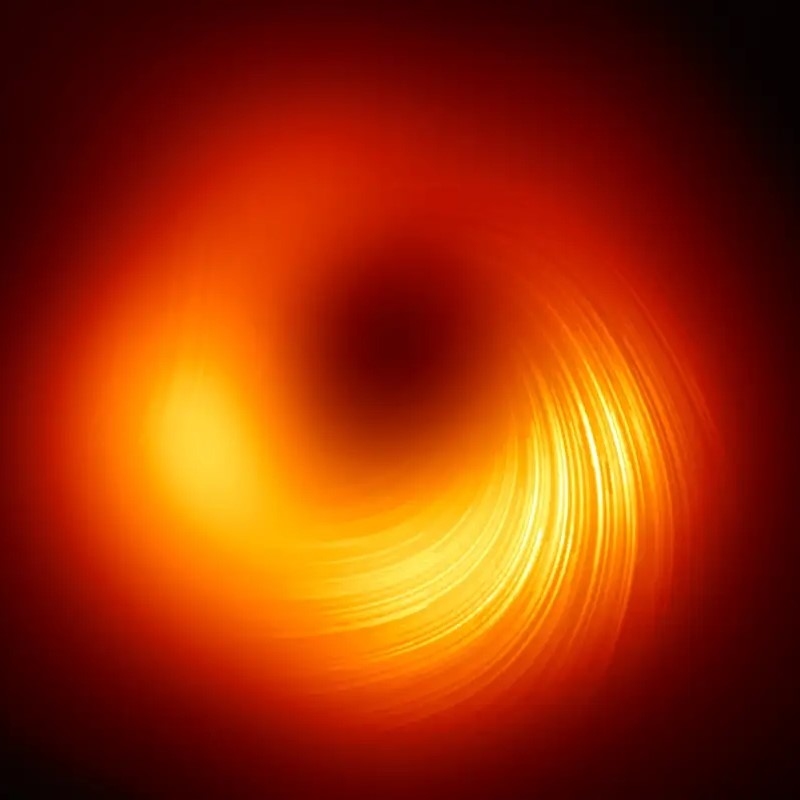
\includegraphics[width=0.5\linewidth]{src/bh_square}
		\caption{Selected image for simulation}
		\label{fig:bhsquare}
	\end{figure}
	
	Different images gave similar results if they followed the conditions cited above.\\
	
	Data simulation will be done as stated in \cite{TER}. First the visibilities matrix is computed using the reference image and the UV-plane of the antenna mesh. To simulate visibilities at different snapshots, we apply the wanted transformation without noise and use the same UV-plane matrix to compute visibilities.\\
	
	To add noise, a normally distributed random matrix is generated and the covariance of that matrix is added to the visibilities one. This matrix could also be directly generated using Wishart distribution. \\ 
	
	\subsection{Reconstruction}
	
	To obtain the initial image $\x_0$ two methods are used depending on the goal of the measure. \\
	
	When reviewing performances under certain errors, all other inputs of the filter - including $\x_0$ - must be errorless. The simplest way of doing that for $\x_0$ is to use the reference image as input. \\
	
	When reviewing Kalman filter performances under real conditions, the reference image is not considered as knwon, and we need to reconstruct the image from the visibilities matrix. While different methods exist \cite{TER}, the ones used here are MVDR reconstructions followed by Maximum Entropy deconvolution.
	
	\newpage
	\part{Reliability of Kalman Filter under perturbations}
	\section{Perturbations sources}
	
	In radio astronomy, many factors can and will affect measures. Those can be :
	\paragraph{Initialisation error} : Kalman filtering requires initializing the first image and the first correlation matrix. Those cannot be exact and will present errors. \\
	Concerning the initial image, multiple precise and efficient methods exist \cite{bible}, and from this initial image the initial correlation matrix can ben initialised\cite{intro_KF} with precision as 
	\begin{equation}\label{p0}
		\P_0 = \autocorr{\x_0} - \moy{\x_0}\moy{\x_0}^H
	\end{equation}
	
	\paragraph{Error covariance matrices} : as mentioned above, these matrices set can be estimated with good accuracy using ALS algorithms [CITATION NEEDED]. It is to be noted that errors on these matrices will not induce new errors in the estimated images, as they are only used to compute the Kalman gain. This implies that inaccurate error matrices can only spread already existing errors on estimated images.
	
	\paragraph{Antennas informations} : Multiple equations in Kalman filtering relies on the observation model $\H$, which is computed as the UV plane FFT covered by the antenna mesh. The limited knowledge of this mesh can create errors in $\H$, particularly when antennas positions and directions cannot be perfectly measured.
	
	\paragraph{Ionospheric perturbations} : Radio astronomical observations can be affected by the passage of the observed electromagnetic waves through the ionosphere \cite{iono}. This can affect the observation model $\H$ as it modifies the perceived direction of the electromagnetic wave measured, and calibration or correction must be made to compensate these perturbations.
	
	\section{Effects of perturbations}
	
	These perturbations create errors on the matrices used in reconstruction and prediction with Kalman filtering. The goal of this part is to evaluate how much these error affect prediction and reconstruction, to determine if Kalman filtering can be realistically used in radio-astronomic context. \\
	
	\subsection{Methodology details}

	First the basic parameters and matrices are computed : antenna grid, directions cosines, baseline vectors.\\ Next, perfect base matrices are computed : errorless observation matrix $\H$, reference observations using the errorless $\H$, error covariance matrices. The latter are computed perfectly using known simulated noise, and errors from ALS estimation are neglected. A set of perfect images are also computed to measure reconstruction absolute error.\\
	Initial image $\x_0$ and covariance $\P_0$ are computed as stated in equation (\ref{p0}).\\
	
	The next step is the generation of an inaccurate matrix normally distributed around the true one - position or direction here. From this matrix is generated an inaccurate  $\H^*$ observations matrix if needed, and Kalman filter is run two times, the first using perfect parameters and the second one using inaccurate ones. In order to smooth out random noise effects this step is repeated 100 times. \\
	
	We can then get the mean error values, measured using a distance defined above, and standard deviations needed.
	
	\subsection{Position}
	
	The first error studied is the position error. A normally distributed error $\vbeps$ is introduced on the antennas positions matrix, giving :
	
	$$
		\z_k^* = \z_k + \vbeps_k
	$$
	
	The new inaccurate baseline is :
	$$
		\dz_{ij}^* = \z_i + \vbeps_i - \z_j - \vbeps_j = \dz_{ij} + \vbeps_{ij}
	$$
	
	The new inaccurate observations matrix's expression is the following :
	\begin{equation}
		\H_{j,q}^* = \exp(-i\frac{2\pi}{\lambda}\dz_{j}^*\dotproduct\I_q) = \exp(-i\frac{2\pi}{\lambda}\left(\dz_{j} + \vbeps_j\right)\dotproduct\I_q) = \exp(-i\frac{2\pi}{\lambda}\dz_{j}\dotproduct\I_q)\exp(-i\frac{2\pi}{\lambda}\vbeps_j\dotproduct\I_q)
	\end{equation}

	The distortion matrix $\C$ can thus be defined such as :
	\begin{equation}
		\H^* = \H\odot\C 
	\end{equation}

	By the same calculation than before \cite{intro_KF}, position error being decorrelated with other errors or noise, the equations become :
	\begin{subequations}
		\begin{equation}\label{xpe}
			\xp^* = \A\xa + \moy{\w_k}
		\end{equation}\begin{equation}
			\yp^* = \H^*\xp^* + \moy{\v_k}
		\end{equation}\begin{equation}
			\Pp^* = \A\Pa^*\A^H + \Q_k
		\end{equation}\begin{equation}
			\K_k^* = \Pp^*\left(\H^*\right)^H\left(\H^*\Pp^*\left(\H^*\right)^H\right)^{-1}
		\end{equation}\begin{equation}
			\Pe^* = \Pp^* + \K_k^*\H^*\Pp^*\left(\H^*\right)^H\left(\K_k^*\right)^H + \K_k^*\R_k\left(\K_k^*\right)^H
		\end{equation}\begin{equation}\label{finKal}
			\xe^* = \xp^* + \K_k^*(\y_k - \yp^*)
		\end{equation}
	\end{subequations}

	To evaluate reconstruction quality, we can introduce the following errors :
	\begin{equation}
		\vbeps^{\K}_k = \K_k^* - \K_k
	\end{equation}
	\begin{equation}\label{errX}
		\vbeps^{\x}_k = \xe^* - \xe
	\end{equation}

	Respectively gain error and estimation error.\\
	Using equation (\ref{xpe}), (\ref{errX}) can be rewritten :
	\begin{equation}
		\vbeps^{\x}_k = \vbeps^{\K}_k\y_k + \left(\mathbb{I} - \K_k^*\H^*\right)\xp^* - \left(\mathbb{I} - \K_k\H\right)\xp
	\end{equation}
	
	In order to measure the performances under positional inaccuracies, the distance $d_1$ is used to evaluate the error between matrices and images :
	\begin{itemize}
		\item Reconstruction error : 
		$$
			\varepsilon_k^{\x} = d_1\left(\xe^*,\x_k\right)
		$$
		\item Additional error : 
		$$
			\varepsilon_k^{\x\x} = d_1\left(\xe^*,\xe\right)
		$$
	\end{itemize}

	Even if $\{\x_k\}$ are real numbers, computing $\{\xe\}$ using $\H$ yields complex matrices. This induces that these errors are not ordered : we can get results like $\varepsilon_k^{\x} < \varepsilon_k^{\x\x}$. 
	Computing these equations gives the following results :
	
	% figures
	
	\begin{figure}[H]
		\centering
		\begin{subfigure}{.5\textwidth}
			\centering
			\includesvg[width=.9\linewidth]{graphs/positions_x_e.svg}
			\caption{Distance to true image}
			\label{fig:p_e_x_e}
		\end{subfigure}%
		\begin{subfigure}{.5\textwidth}
			\centering
			\includesvg[width=.9\linewidth]{graphs/positions_xx.svg}
			\caption{Distance to "perfect" reconstruction}
		\end{subfigure}
	\caption{Simulation results for positional inaccuracy}
	\end{figure}
	
	% discussion
	For these simulations, reconstruction error without inaccuracies is 
	$$ % expval ? => ptet mettre <.> ?
	\left\langle d_1\left(\xe,\x_k\right)\right\rangle = 8,46\times10^{-4}
	$$
	and is represented by the blue line in (\ref{fig:p_e_x_e}).\\
	
	The first interesting observations on these graphs are the extremities convergences : above 0,05m position error standard deviation, errors approach a distance of 0,1. The $d_1$ distance being normalised (as $\x$ and $\xe$ are normalised between 0 and 1), this distance means 10\% reconstruction error. This error level represents non reliable reconstruction. It can be illustrated by the following reconstruction :
	\begin{figure}[H]
		\centering
		\begin{subfigure}{.5\textwidth}
			\centering
			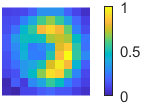
\includegraphics[width=.7\linewidth]{src/t_im.png}
			\caption{True image}
		\end{subfigure}%
		\begin{subfigure}{.5\textwidth}
			\centering
			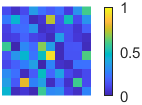
\includegraphics[width=.7\linewidth]{src/t_err.png}
			\caption{Reconstruction at 0,1 distance of the true image}
		\end{subfigure}
		\caption{Image reconstruction at unreliable distance}
	\end{figure}

	This distance around 0,1 is actually expected, as the mean distance $d_1$ between two random matrices in $\mathcal{M}_{10}([0;1])$ can be computed and gives 1,167. The random effects of position errors getting more important, the reconstruction using this inaccurate positions matrix is becoming random thus converging to this value of 1,167.
	
	\subsection{Direction}
	
	Direction error can be caused by a misaligned antenna, or a small displacement, but will mostly come from ionospheric perturbation\cite{iono}. To study the effects of these perturbations, a normally distributed error $\vbeps$ is introduced on the direction matrix :
	
	\begin{equation}
		\I_q^* = \I_q + \vbeps_q
	\end{equation}

	The observations matrix becomes :
	$$
		\H_{j,q}^* = \exp(-i\frac{2\pi}{\lambda}\dz_{j}\dotproduct\I_q^*) = \exp(-i\frac{2\pi}{\lambda}\dz_{j}\dotproduct\I_q)\exp(-i\frac{2\pi}{\lambda}\dz_{j}\dotproduct\vbeps_q)
	$$
	A directional distortion matrix can be defined such as :
	\begin{equation}
		\H^* = \H \odot \D
	\end{equation}

	Kalman equations from (\ref{xpe}) to (\ref{finKal}) stay the same.\\
	
	To further measure the effect of this error, it will be introduced on a single direction first, then on all of them. 
	
	\subsubsection{One direction}
	
	\subsubsection{All directions}
	
	\newpage
	\part{Experimental correction}
	\section{implementation}
	\section{Measures}
	
	\newpage
	\part{Further insights}
	
	% err dir 1 antenne plutôt que sur 1 dir
	% smoother
	% deep
	
	\paragraph{Directional error on one antenna :} on larger arrays, ionospheric perturbations might not affect all antennas the same, thus studying the reliability when one antenna has errors might be an idea to explore.
	
	\paragraph{Use of smoothers :} when using a Kalman filter, only prior knowledge of data is needed. When all measures at different snapshots are done, a \emph{smoother}\cite{RTS} can be used to give better Kalman results, their reliability under perturbations needs to be discussed. 
	
	\paragraph{Deep learning :} In image processing, deep learning and artificial intelligence are getting more effective and reliable. In particular, model based deep learning \cite{deep} can be an effective way of rebuilding images when an evolution model is known.
	
	\newpage
	\printbibliography
\end{document}

\begin{figure}[H]
	\centering
	\includegraphics[width=0.7\linewidth]{}
	\caption{}
\end{figure}

\begin{figure}[H]
	\centering
	\begin{subfigure}{.5\textwidth}
		\centering
		\includegraphics[width=.4\linewidth]{image1}
		\caption{}
	\end{subfigure}%
	\begin{subfigure}{.5\textwidth}
		\centering
		\includegraphics[width=.4\linewidth]{image2}
		\caption{}
	\end{subfigure}
	\caption{}
\end{figure}
